%%%%%%%%%%%%
%
% $Autor: Wings $
% $Datum: 2019-03-05 08:03:15Z $
% $Pfad: TemplateSensor $
% $Version: 4250 $
% !TeX spellcheck = en_GB/de_DE
% !TeX encoding = utf8
% !TeX root = filename 
% !TeX TXS-program:bibliography = txs:///biber
%
%%%%%%%%%%%%

% Structure
\chapter{Drehpotentiometer}

%Notizen:

%Drehpotentiometer
%Widerstand 10 kOhm, linear
%Achse 6 mm 
%Spannungsfestigkeit: 250 VDC	
%Befestigung Gewinde M10
%
%{../../Images/BOM/Drehpotentiometer_10kOhm_linear_6mm.jpg} 
%
%https://www.reichelt.de/de/de/shop/produkt/drehpotentiometer_10_kohm_linear_6_mm-232554

\section{Allgemeines}
\label{sec:AllgPoti}
Der potentiometrische Wandler auf Basis eines gleitend-reibenden Kontaktelements auf
einer elektrischen Widerstandsbahn wird in Kurzform Potentiometer genannt. \cite{Czechowicz:2025}
Wie in Abbildung \ref{pic:PotiRotLin} drehbare- und lineare Potentiometer eingesetzt, mit denen respektiv Stellwinkel oder Stellwege erfasst werden können. \cite{Czechowicz:2025}

\begin{center}
	\begin{figure}
		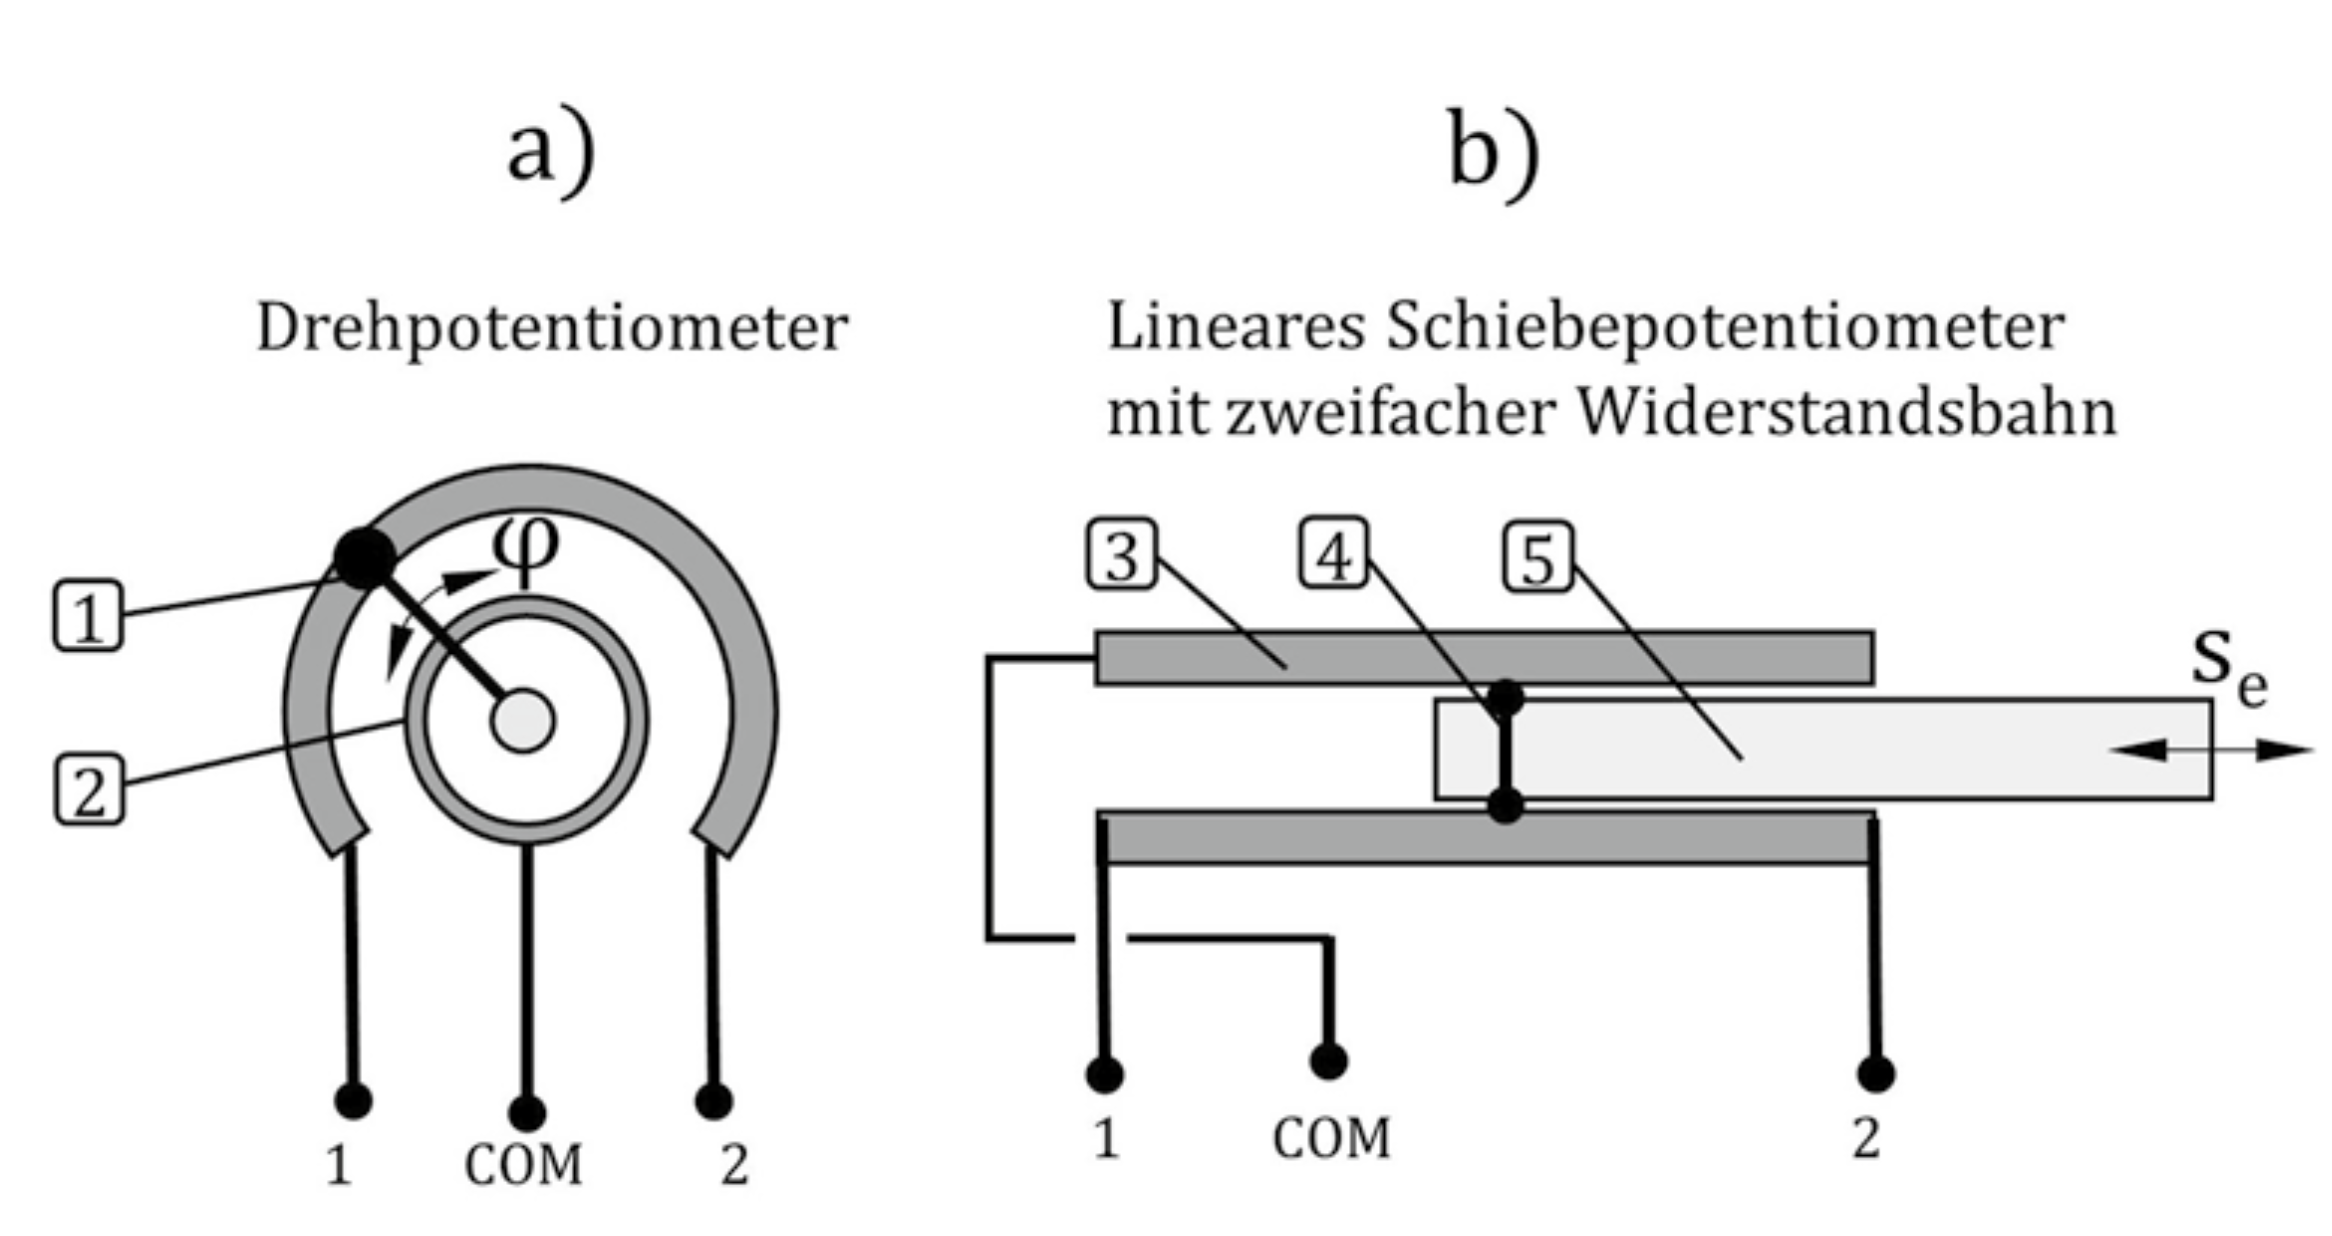
\includegraphics[scale=0.25]{../../Images/PC16/UebersichtPotentiometer.png}
		\caption{Bauformen von Potentiometern nach \cite{Czechowicz:2025}} 
		\label{pic:PotiRotLin}
	\end{figure}
\end{center}

Mit Hilfe des variablen Widerstands eines Potenziometers lässt sich ein Spannungsteiler realisieren, bei dem die Spannungsteilung einstellbar ist. \cite{Meier:2022}

\section{Drehpotentiometer PIHER PC-16}

Das Drehpotentiometer PC-16 ist ein 16 mm Carbon-Potentiometer zur Montage auf Bedienpaneelen. \cite{PIHER:2024}
Aufgrund seiner schlanken Bauweise eignet es sich hervorragend zum einbau in kleineren Elektrogeräten.
Das Drehpotentiometer soll beim elektrischen Tischförderband zur Vorwahl der Bandgeschwindigkeit eingesetzt werden.

\section{Spezifikationen}

\begin{center}
	\begin{figure}
		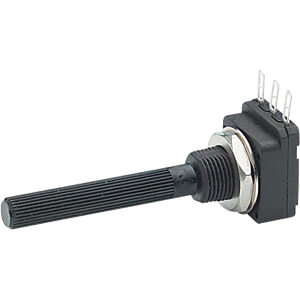
\includegraphics[scale=0.25]{../../Images/BOM/Drehpotentiometer10kOhm.jpg}
		\caption{Drehpotentiometer PIHER PC16 nach (QUELLE)} 
		\label{pic:POTI10k}
	\end{figure}
\end{center}

\begin{table}[h!]
	\caption{Spezifikationen des Drehpotentiometers (PC-16 - 16mm panel mount potentiometer, 2026)}
	\begin{center}
		\begin{tabular}{|l|l|}
			\hline
			\textbf{Parameter} &\textbf{Wert/Detail}\\
			\hline
			Modell & PC16SH-10CP06-103A2020-TA\\
			\hline
			Typ  & Drehpotentiometer\\
			\hline 
			Widerstand & 10 $k\Omega$, linear\\
			\hline
			Nennlast & 0,2 $W$\\ 
			\hline 
			Spannungsfestigkeit & 250 $V$\\
			\hline
			Drehwinkel & 300 °\\
			\hline
			Achse & 6 $mm$\\
			\hline 
			Befestigung & Gewinde M10\\
			\hline 
			Max. Betriebstemperatur & 70 °C\\
			\hline 
			
		\end{tabular}
		\label{TabelleSpezifikationPOTI}
	\end{center}
\end{table} 


Das Drehpotentiometer besitzt wie in Abbildung \ref{pic:POTI10k} erkenntlich drei Anschlüsse. Diese Anschlüsse können wie folgt beschrieben werden: 
\begin{enumerate}
		\item \textbf{A}: Spannungsanschluss 1
		\item \textbf{S}: Signalanschluss
		\item \textbf{E}: Spannungsanschluss 2
\end{enumerate}
Diese Anschlüsse A und E beschreiben die Endlagen des jeweiligen Potentiometers, der Anschluss S beschreibt den Signalanschluss, der abhängig von der Stellung des Schaftes . Die Polung der Anschlüsse ist Bauart und Anwendungsabhängig.

\section{Bibliothek}
Für die Verwendung eines einfachen Drehpotentiometers mit drei Anschlüssen wird in der Regel keine zusätzliche Bilbiothek benötigt.

\section{Anwendungsbeispiel}
\label{sec:AnwendungPC16}
Das Drehpotentiometer lässt sich mit kleinem Aufwand anschließen. Man kann es sowohl in analogen Schaltkreisen wie in \ref{sec:AllgPoti} Allgemeines als variablen Widerstand oder Spannungsteiler verwenden, als auch als analogen Signalgeber an einem Mikrocontroller.
Das folgende Anwendungsbeispiel demonstriert den Anschluss an einem Arduino mit eingebauter LED und nutzt das Drehpotentiometer, um das Leuchtverhalten der LED zu steuern.

\begin{center}
	\begin{figure}
		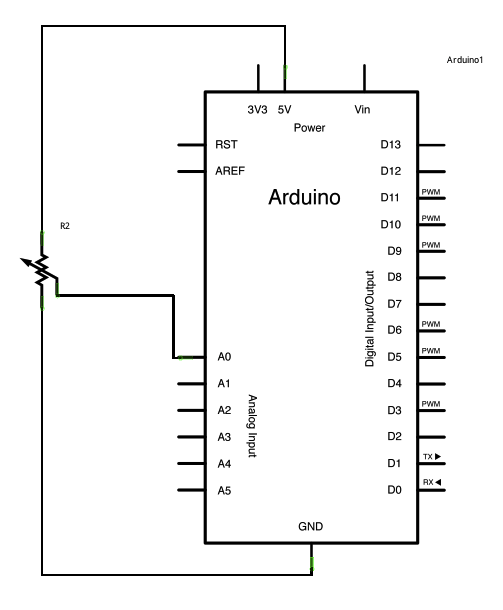
\includegraphics[scale=0.35]{../../Code/Potentiometer/AnalogInput/schematic}
		\caption{Anschlussbeispiel des PC16 nach \cite{ArduinoAnalog:2026}} 
		\label{pic:PC16Anschluss} 
	\end{figure}
\end{center}

\subsection{Einfacher Funktionstest}
Um die Ordnungsgemäße Funktion des Drehpotentiometers sicherzustellen, ist es sinnvoll dieses vor der Verwendung zu testen. Hierfür kann die in \ref{pic:PC16Anschluss} gezeigte Schaltung verwendet werden. Um die Funktion des Drehpotentiometers am Arduino zu prüfen kann folgendes Vorgehen befolgt werden: 

\begin{center}
	\begin{enumerate}
		\item Alle Anschlüsse und Verbindungen nach \ref{pic:PC16Anschluss} verbinden und auf festen Sitz prüfen. 
		\item Den Arduino mit einem Computer VerbindenSpannungsversorgung (12V) einschalten.   
		\item Prüfen ob der Motor sich mit konstanter Drehzahl dreht. 
	\end{enumerate}  
\end{center}

\section{Einfacher Code}
Um das Signal des Drehpotentiometers verarbeiten und intepretieren zu können muss das Signal durch den Mikrocontroller eingelesen und anschließend ausgewertet werden. Der Code \ref{CodeAnschlussPC16} von \cite{ArduinoAnalog:2026} zeigt eine mögliche Umsetzung. 

Zu Beginn dieses Sketches wird die Variable \python{sensorPin} auf den Analog-Pin 0 gesetzt, an dem das Drehpotentiometer angeschlossen ist. Der Ausgang \python{ledPin} wird auf den Digital-Pin 13 gesetzt. Außerdem wird eine weitere Variable \python{sensorValue} definiert, um die vom Sensor gelesenen Werte zu speichern.
Der Befehl \python{analogRead()} wandelt den Eingangsspannungsbereich von 0 bis 5 Volt in einen digitalen Wert zwischen 0 und 1023 um. Dies geschieht durch eine Schaltung im Mikrocontroller, die als Analog-Digital-Wandler oder ADC bezeichnet wird.
Durch Drehen der Welle des Drehpotentiometers verändern sich die relativen Widerstände zwischen dem Signalanschluss und den beiden äußeren Anschlüssen, wodurch Sie eine variable Spannung am Analogeingang erhalten. Wenn die Welle ganz in eine Richtung gedreht wird, besteht kein Widerstand zwischen dem Signalanschluss und dem mit Masse verbundenen Stift. Die Spannung am Signalanschluss beträgt dann 0 Volt und \python{analogRead()} gibt 0 zurück. Wenn die Welle ganz in die andere Richtung gedreht wird, besteht kein Widerstand zwischen dem Signalanschluss und dem mit +5 Volt verbundenen Anschluss. 
Die Spannung am Signalanschluss beträgt dann 5 Volt, und \python{analogRead()} gibt den Wert 1023 zurück. Dazwischen gibt \python{analogRead()} einen Wert zwischen 0 und 1023 zurück, der proportional zur am Pin anliegenden Spannung ist.
Dieser Wert, der in \python{sensorValue} gespeichert ist, wird verwendet, um eine \python{delay()} für den Blinkzyklus festzulegen. Je höher der Wert, desto länger der Zyklus; je kleiner der Wert, desto kürzer der Zyklus. Der Wert wird zu Beginn des Zyklus gelesen, daher ist die Ein- und Ausschaltzeit immer gleich.


\begin{center}
	\captionof{figure}{Mit der Arduino IDE gelieferter Code zum Testen analoger Eingänge \cite{ArduinoAnalog:2026}} 
	\label{CodeAnschlussPC16}
	\ArduinoExternal{}{../../Code/Potentiometer/AnalogInput/AnalogInput.ino}
\end{center}

\section{weiterführende Literatur} 
\begin{center}
	\begin{enumerate}
		
		%Hier Literatur anfügen
		
	\end{enumerate}
\end{center}

